\documentclass[14pt]{beamer}
\usepackage{listings}
\usepackage{inconsolata}
\usepackage[T1]{fontenc}
\usepackage[scaled]{helvet}
\renewcommand*\familydefault{\sfdefault}

\usetheme{Boadilla}
\usecolortheme{orchid}

\lstset{
  basicstyle=\ttfamily\footnotesize,
  showspaces=false,
  showstringspaces=false
}

\title{Using OpenStreetMap data with Python}
\author{Andrii V. Mishkovskyi}
\date{\today}

\AtBeginSection[]{%
  \begin{frame}<beamer>
    \begin{center}
      \LARGE{\tableofcontents[sectionstyle=show/hide,
      subsectionstyle=hide/show/hide]}
    \end{center}
  \end{frame}
}

\begin{document}

\begin{frame}
  \titlepage
\end{frame}

\begin{frame}
  \frametitle{Who is this dude anyway?}
  \begin{itemize}
  \item I love Python
  \item I love OpenStreetMap
  \item I do map rendering at CloudMade using Python
  \item CloudMade uses OpenStreetMap data extensively
  \end{itemize}
\end{frame}

\section*{Introduction}

\begin{frame}
  \frametitle{Objectives}
  \begin{itemize}
  \item Understand OpenStreetMap data structure
  \item How to parse it
  \item Get a feel of how basic GIS services work
  \end{itemize}
\end{frame}

\begin{frame}
  \frametitle{OpenStreetMap}
  \begin{itemize}
  \item Founded in 2004 as a response to Ordnance
    Survey pricing scheme
  \item >400k registered users
  \item >16k active mappers
  \item Supported by Microsoft, MapQuest (AOL), Yahoo!
  \item Crowd-sourcing at its best
  \end{itemize}
\end{frame}

\begin{frame}
  \frametitle{Why OSM?}
  \begin{itemize}
  \item Fairly easy
  \item Good quality
  \item Growing community
  \item Absolutely free
  \end{itemize}
\end{frame}

\section{Data layout}

\begin{frame}[fragile]
  \begin{center}
    
\includegraphics[width=300px]{introduction.jpg}
  \end{center}
\end{frame}

\begin{frame}
  \frametitle{Storage type}
  \begin{itemize}
  \item XML (.osm)
  \item Protocol buffers (.pbf, in beta status)
  \item Other formats through 3rd parties
    (Esri shapefile, Garmin GPX, etc.)
  \end{itemize}
\end{frame}

\begin{frame}
  \frametitle{The data}
  \begin{itemize}
  \item Each object has geometry, tags and changeset information
  \item Tags are simply a list of key/value pairs
  \item Geometry definition differs for different types
  \item Changeset is not interesting when simply using the
    data (as opposed to editing)
  \end{itemize}
\end{frame}

\begin{frame}
  \frametitle{Data types}
  \begin{description}
  \item[Node] Geometric point or point of interest
  \item[Way] Collection of points
  \item[Relation] Collections of objects of any type
  \end{description}
\end{frame}

\begin{frame}
  \frametitle{Nodes}
  \center{\lstinputlisting[language=XML]{nodes.xml}}
\end{frame}

\begin{frame}
  \frametitle{Ways}
  \only<1>{\center{\lstinputlisting[language=XML]{ways.xml}}}
\end{frame}

\begin{frame}
  \frametitle{Relations}
  \only<1>{\lstinputlisting[language=XML]{relations.xml}}
\end{frame}

\section{Importing}

\begin{frame}[fragile]
  \begin{center}
    
\includegraphics[width=300px]{surprised.png}
  \end{center}
\end{frame}

\begin{frame}
  \frametitle{Major points when parsing OSM}
  \only<1>{
    \begin{itemize}
    \item Expect faulty data
    \item Parse iteratively
    \item Cache extensively
    \item Order of elements is not guaranteed
    \item But it's generally: nodes, ways, relations
    \item Ids are unique to datatype, not to the whole data set
    \end{itemize}
  }
\end{frame}

\begin{frame}
  \frametitle{Parsing data}
  \begin{itemize}
    \item Using SAX
    \item Doing simple reprojection
    \item Create geometries using Shapely
  \end{itemize}
\end{frame}

\begin{frame}
  \frametitle{Parsing data}
  \framesubtitle{Projection}
  \lstinputlisting[language=Python]{projection.py}
\end{frame}

\begin{frame}
  \frametitle{Parsing data}
  \framesubtitle{Nodes}
  \only<1>{\lstinputlisting[language=Python]{nodes.py}}
  \only<2>{
    \lstinputlisting[firstline=1,lastline=16,language=Python]{nodes-simple.py}
  }
  \only<3>{
    \lstinputlisting[firstline=17,language=Python]{nodes-simple.py}
  }
\end{frame}

\begin{frame}
  \frametitle{Parsing data}
  \framesubtitle{Ways}
  \only<1>{\lstinputlisting[language=Python]{ways.py}}
  \only<2>{
    \lstinputlisting[firstline=1,lastline=14,language=Python]{ways-simple.py}
  }
  \only<3>{
    \lstinputlisting[firstline=15,language=Python]{ways-simple.py}
  }
\end{frame}

\begin{frame}
  \frametitle{Parsing data}
  \framesubtitle{Relations}
  \only<1>{\lstinputlisting[language=Python]{relations.py}}
  \only<2>{
    \begin{center}
      \Large{The importing code is left as an exercise for the reader}
    \end{center}
  }
\end{frame}

\begin{frame}
  \frametitle{For language zealots}
  \begin{center}
    \LARGE{Excuse me for not using namedtuples.}
  \end{center}
\end{frame}

\begin{frame}
  \frametitle{Parsing data: homework}
  \begin{itemize}
  \item The idea is simple
  \item The implementation can use ElementTree if you work with
    small extracts of data
  \item Have to stick to SAX when parsing huge extracts or
    the whole planet data
  \end{itemize}
\end{frame}

\begin{frame}
  \frametitle{Existing solutions}
  \begin{itemize}
  \item Osmosis
  \item osm2pgsql
  \item osm2mongo, osm2shp, etc.
  \end{itemize}
\end{frame}

\section{Rendering}

\begin{frame}[fragile]
  \begin{center}
    
\includegraphics[width=300px]{map.jpg}
  \end{center}
\end{frame}

\begin{frame}
  \frametitle{Principles}
  \begin{itemize}
  \item Scale
  \item Projection
  \item Cartography
  \item Types of maps
  \end{itemize}
\end{frame}

\begin{frame}
  \frametitle{Layers}
  \begin{itemize}
  \item Not exactly physical layers
  \item Layers of graphical representation
  \item Don't render text in several layers
  \end{itemize}
\end{frame}

\begin{frame}
  \frametitle{How to approach rendering}
  \begin{itemize}
  \item Split your data in layers
  \item Make projection configurable
  \item Provide general way to select data sources
  \item Think about cartographers
  \end{itemize}
\end{frame}

\begin{frame}
  \frametitle{The magic of Mapnik}
  \lstinputlisting[language=Python]{mapnik-overview.py}
\end{frame}

\begin{frame}
  \frametitle{Magic?}
  \begin{itemize}
  \item Mapnik's interface is straightforward
  \item The implementation is not
  \item Complexity is hidden in XML
  \end{itemize}
\end{frame}

\begin{frame}
  \frametitle{Mapnik's XML}
  \only<1>{
    \lstinputlisting[language=XML]{mapnik-style.xml}
  }
  \only<2>{
    \lstinputlisting[language=XML]{mapnik-layer.xml}
  }
\end{frame}


\section{Searching}

\begin{frame}[fragile]
  \begin{center}
    
\includegraphics[width=300px]{geocoding.jpg}
  \end{center}
\end{frame}

\begin{frame}
  \frametitle{What's that?}
  \begin{itemize}
  \item Codename geocoding
  \item Similar to magnets
  \item Fast or correct -- choose one
  \end{itemize}
\end{frame}

\begin{frame}
  \frametitle{Why is it hard?}
  \only<1>{
    \begin{itemize}
    \item Fuzzy search
    \item Order matters
    \item But not always
    \item One place can have many names
    \item One name can correspond to many places
    \item People don't care about this at all!
    \end{itemize}
  }
  \only<2>{
    \begin{center}
      \LARGE{I blame Google.}
    \end{center}
  }
\end{frame}

\begin{frame}
  \frametitle{Attempt at implementation}
  \only<1>{
    \begin{itemize}
    \item Put restrictions
    \item Make the request structured
    \item Or at least assume order
    \item Assume valid input from users
    \end{itemize}
  }
  \only<2>{
    \lstinputlisting[language=Python]{structured-geocoding-prototype.py}
  }
\end{frame}

\begin{frame}
  \frametitle{Fixing user input}
  \only<3>{
    Edit distance
    \begin{itemize}
    \item Works for two words
    \item Most geocoding requests consist of several words
    \item Scanning database for each pair distance isn't feasible
    \item Unless you have it cached already
    \item Check out Peter Norvig's
      ``How to Write Spelling a Corrector'' article
    \end{itemize}
  }
  \only<1>{
    Soundex/Metaphone/DoubleMetaphone
    \begin{itemize}
    \item Phonetic algorithms
    \item Works in 90\% of the cases
    \item If your language is English
    \item Doesn't work well for placenames
    \end{itemize}
  }
  \only<2>{
    \lstinputlisting[language=Python]{geocoding-soundex.py}
  }
  \only<4>{
    N-grams
    \begin{itemize}
    \item Substrings of n items from the search string
    \item Easier to index than edit distance
    \item Gives less false positives than phonetic algorithm
    \item Trigrams most commonly used
    \end{itemize}
  }
  \only<5>{
    \lstinputlisting[language=Python]{geocoding-trigrams.py}
  }
\end{frame}

\begin{frame}
  \frametitle{Making the search free-form}
  \only<1>{
    \begin{itemize}
    \item Normalize input: remove the, a, \ldots
    \item Use existing free-form search solution
    \item Combine ranks from different sources
    \end{itemize}
  }
  \only<2>{
    \lstinputlisting{geocoding-freeform.py}
  }
\end{frame}

\section{Routing}

\begin{frame}[fragile]
  \begin{center}
    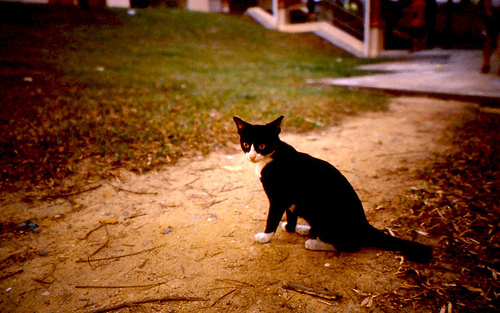
\includegraphics[width=300px]{routing.jpg}
  \end{center}
\end{frame}

\begin{frame}
  \frametitle{The problem}
  \only<1>{
    When introduced with routing problem, people think
    Build graph, use Dijsktra, you're done!
    (And they are mostly right)
  }
  \only<2>{
    Not that simple
    \begin{itemize}
    \item Graph is sparse
    \item Graph has to be updated often
    \item Dijkstra algorithm is too general
    \item A* is no better
    \end{itemize}
  }
  \only<3>{
    \begin{itemize}
    \item Routing is not only a technical problem
    \item Different people expect different results for the same input
    \item Routing through cities is always a bad choice
      (even if it's projected to be faster)
    \end{itemize}
  }
\end{frame}

\begin{frame}
  \frametitle{Building the graph}
  \only<1>{
    \begin{itemize}
    \item Adjacency matrix is not space-efficient
    \item The graph representation has to very compact
    \item networkx and igraph are both pretty good for a start
    \end{itemize}
  }
  \only<2>{
    \lstinputlisting[language=Python]{routing-networkx.py}
  }
  \only<3>{
    \begin{itemize}
    \item There is no silver bullet
    \item No matter how nice these libs are, importing even
      Europe will require more than 20 GB of RAM
    \item Splitting data into country graphs is not enough
    \item Our in-house C++ graph library requires ~20GB
      of mem for the whole world
    \end{itemize}
  }
\end{frame}


\begin{frame}
  \frametitle{Other solutions}
  \begin{itemize}
  \item PgRouting -- easier to start with, couldn't make it fast,
    harder to configure
  \item Neo4j -- tried 2 years ago, proved to be lacking when
    presented with huge sparse graphs
  \item Eat your own dogfood -- if doing ``serious business'', most
    probably the best solution. Half-wink.
  \end{itemize}
\end{frame}

\section*{Summary}

\begin{frame}
  \begin{center}
    \only<1>{\LARGE{Bored already?}}
    \only<2>{\LARGE{Lighten up, I'm done}}
  \end{center}
\end{frame}

\begin{frame}
  \frametitle{Highlights}
  \begin{itemize}
  \item Start using OpenStreetMap data -- it's easy
  \item Try building something simple -- it's cool
  \item Try building something cool -- it's simple
  \item Python is one of the best languages [for doing GIS]
  \end{itemize}
\end{frame}

\begin{frame}
  \begin{center}
    \LARGE{Questions?}
  \end{center}
  \vfill
  \begin{center}
    \texttt{contact@mishkovskyi.net}\\
    Slides: \texttt{mishkovskyi.net/ep2011}
  \end{center}
\end{frame}

\end{document}
